%!TEX root = ../dissertation.tex

\chapter{Conclusion}
\label{chapter:conclusion}

\section{General conclusion}
\subsection{Work during internship}
This document presented the solution and the work that has been done during my first semester of my international year in \ref{IST}, in Lisbon, Portugal. During this time, I developed an image based visual servoing that is implemented and is now part of the algorithm data base (github) of the SocRob team. This algorithm is robust and generic, working both in simulation and real robot, with different arm controllers. It has been a real challenge for me to work in this environment, C++, ROS and Linux were not part of original background. I have learn so much during this 6 months. ROS is an environment that takes time to appreciate but when you manage to do it, it is really helpful. From code review, code cleaning, code development it has been an everyday challenge and I am proud of my work. I hope it will be used and served as a base for future work on image based manipulation inside the SocRob team. 
With this work, we enhanced team’s manipulation skills with being able to grasp various types of objects in a dynamic environment.
I have also been able to apply more of my mechanical background by doing some annex work like calibration of the base of the arm using a minimization closed form solution and using Mocap vision system that is present in the laboratory.
With the various testing made, some issues have been point out:
\begin{itemize}
    \item Nothing inside the design of our controller or the inverse kinematic Cartesian controller, keep the feature insight. I have tried to implement it inside the optimization forward kinematic controller with a barrier log function but there are still some issues to solve.
    \item No rotational control makes some grasping approach fail. 
\end{itemize}

\subsection{Future work}
From the issues pointed out from last section, we can defined some future work:
\begin{itemize}
    \item Implementing a 3D grasping estimation algorithm, to be able to control the rotational motions of the manipulator to be able to be more robust when grasping.
    \item Implementing a grasping planner (already on very good track with another student work), this planner will put the arm in a good  grasping configuration and to avoid calibrations issues for the final approach my algorithm could be used.
    \item Improve the inverse kinematic Cartesian controller to add constraints to keep the features insight. 
\end{itemize}

\section{Life in Portugal}

Portuguese life was very nice. I enjoyed it a lot. Lisbon is a very beautiful city with a lots of things to do. You can go hiking, surfing and swimming from less than 30 min from the city but be careful the water is very cold ! The life is still kind of cheap, you can live in Lisbon with less than 900 euros but the price are going up quickly. I was living near the tecnico and could walk every day to get there. \\[2cm]

\begin{figure} [!ht]
    \centering
    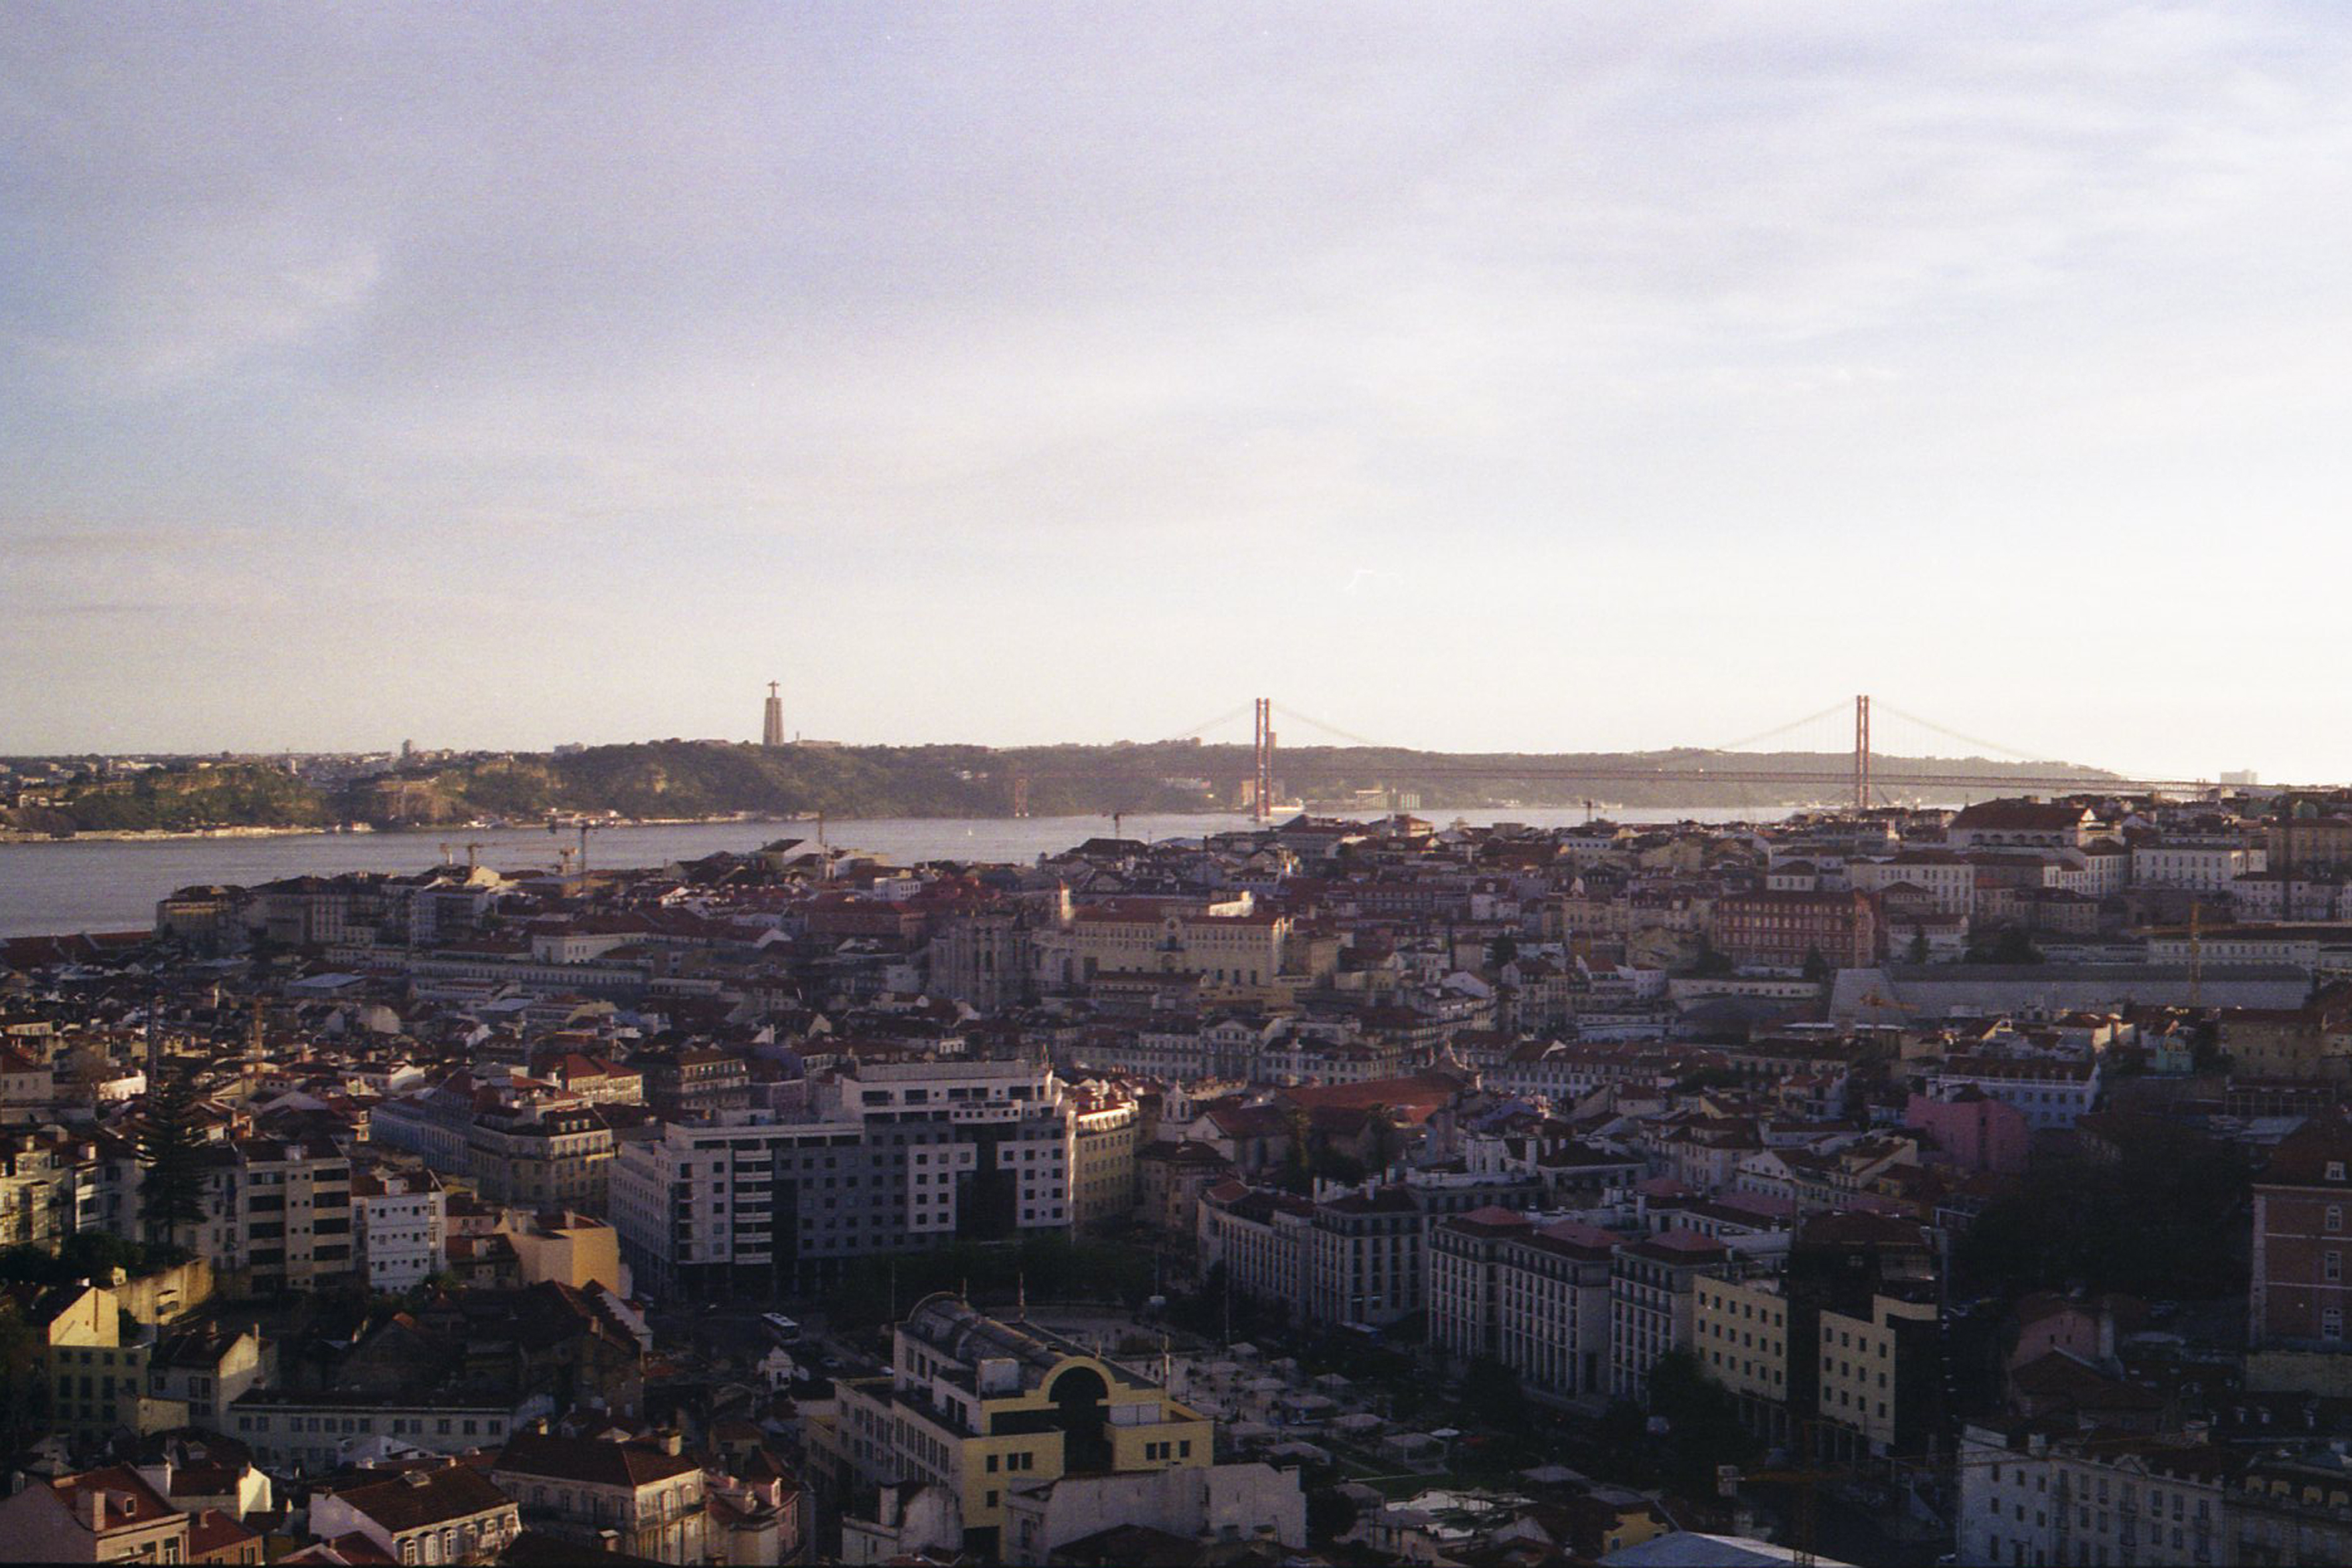
\includegraphics[width=1\linewidth]{images/12.jpg}
    \caption{Lisbon view, not far from my apartment in Anjos !}
    \label{pict:open_loop}
\end{figure}